\chapter{General Discussion}\label{chp:discussion}
Following up on the results presented above, this chapter discusses the most important ones in more detail: Section~\ref{sec:6-disc} focuses on the puzzling effects of diminutive type and its interplay with the other predictors, while Section~\ref{sec:6-limits} discusses the additional methodological and theoretical limitations of the study that could possibly have contributed to the complex picture observed for diminutive type.

\section{Discussion of Results}
\label{sec:6-disc}
A quick glance at the effects predicted by the mixed-effects model establishes surface frequency, orthographic similarity, age of acquisition, and word prevalence as the significant predictors with the most pronounced effects on reaction times. This is in line with the effects observed for each of these predictors in previous literature, most importantly \citeauthor{Brysbaert+etal+2016} (\citeyear{Brysbaert+etal+2016}) as the founding study for the DLP2. The robust replication of these variables' effects points to the reliability of the chosen model and contributes to the credibility of predictions made for all the other variables included in the model. Differences in effect size between the results reported here and in \citeauthor{Brysbaert+etal+2016} can be easily explained by the design of the present study. For example, the formula for the experimental model differs from that used in \citeauthor{Brysbaert+etal+2016} due to being adapted for the study of morphology, while all continuous predictors have been centered and standardised as discussed in Chapter~\ref{chp:study}, framing their effect sizes in different terms compared to the DLP2 paper.

The experimental results for the effect of diminutive type present a complex picture. Taken on its own, the difference between group means is negligible, yet significant, with derivational diminutives taking slightly longer to recognize on average. At first glance, this seems to confirm the expectations for the proposed structural and functional differences between the two types of diminutive to be reflected in behavioral measurements. However, as soon as diminutive type is introduced in a linear regression model alongside the standard predictors, its effect on reaction times is quickly levelled in comparison and fails to achieve significance. This alone indicates that diminutive type as defined in this study is not a strong enough predictor on its own, with the variance it might explain better accounted for by other predictors. Due to the inclusion of an interaction term, the effect of diminutive type alone is uninterpretable; however, one cannot help but observe the model predicting the derivational diminutives to take slightly less time on average, conflicting with the initial observations based on the comparison of means.

By contrast, the predicted effects of the only other morphology-related variable, morpheme count, are independent and therefore immediately interpretable. While reaction times are expectedly predicted to be longer for more internally complex words, morpheme count has a particularly negligible effect size and furthermore fails to achieve significance. In other words, what could have sapped the explanatory power of diminutive type by virtue of reflecting the same underlying structural difference in terms of a continuous variable is instead reported as having a barely observable, non-significant effect on the overall processing times.

The reported interaction effects between frequency and diminutive type further complicate matters. The prediction that the more complex derivational type would take longer to process seems only to apply to diminutives with an above-average frequency of occurrence (more than once per 10.000 words). By contrast, among lower-frequency diminutive words, inflectional forms are predicted to trail behind derivational ones, reflecting the observed effect of diminutive type outside of the interaction term. This pattern is highly unexpected under the working theory: assuming syntax-all-the-way-down coupled with across-the-board full decomposition of every complex form, surface frequency should have little opportunity to majorly modulate the processing of more or less complex structures. Instead, it is the individual frequency of every constituent morpheme making up a particular word that should logically impact decomposition-based processes the most. This point is argued in \citeauthor{Taft+1979} (\citeyear{Taft+1979}), who observes effects of both surface and stem frequency in visual word processing and further comments that the findings in favour of a competing analysis in \citeauthor{Manelis+Tharp+1977} (\citeyear{Manelis+Tharp+1977}) were inconclusive on the basis of \citeauthor{Manelis+Tharp+1977} not matching their stimuli for frequency of their constituent morphemes. However, \citeauthor{Taft+1979} (\citeyear{Taft+1979}) notes that both frequency measures are inherently correlated, as the base frequency of every morpheme is the sum of surface frequencies of every wordform it has been attested to occur in.

For the current analysis, the implication is clear: a complex form like \textit{onderwijzertje} would be decomposed into \textit{onder-}, \textit{-wijz-}, \textit{-er-}, and \textit{-tje}, and the entries for the individual morphemes looked up and accessed based on their respective frequency. Therefore, the cumulative sum of by-morpheme frequencies could heavily impact the total time taken to recognise a word. Every single wordform in this study is additionally suffixed with \textit{-tje}. As the suffix is assumed to have a single representation, albeit multiple morphological functions, its frequency is held constant between the two conditions. This lends greater influence to the frequencies of the remaining constituent morphemes, e.g. the root(s) and other affixes. With surface and base frequencies previously attested to correlate, it could be that the interaction effect observed for the Zipf-transformed surface frequency is in fact the effect of base frequencies of individual morphemes.

Unfortunately, there is no easy way to confirm or deny this proposition: base frequency is not a variable included in the original makeup of the DLP2, and thus the corpus itself cannot be relied upon to provide the information necessary to disentangle the frequency effects. In addition, taking into account the base frequency of every constituent morpheme is difficult for complex forms such as \textit{onderwijzertje}; the only way to control for base frequency effects seems to be by subtracting the base frequency value of \textit{-tje} from the cumulative base frequency for every word. However, this option, too, relies on the relevant information being present in the corpus, and is non-implementable within the limitations of the current work.

Note, as well, that the effect size of the interaction term is decidedly lower than that of any other significant predictor, and it achieves only marginal significance with the $p$-value lying rather close to the alpha-threshold of 0.05. This shows that even an interaction term such as this explains barely enough variance to warrant rejecting the null hypothesis of it having no effect whatsoever on lexical decision. Furthermore, with the distance between slopes at the mean frequency value of 1 per 10.000 words being very close as reflected in Figure~\ref{fig:interaction}, the difference between the two groups within the average surface frequency range is marginal at best. Taking all of this into consideration, the effects of surface frequency interactions with diminutive type are inconclusive. The silver lining of this observation is that the functional split proposal has not been refuted outright, with the predicted effects possibly being artifacts of experimental design.

All in all, the effects of diminutive type observed in the experimental study, while not conclusive at all, serve as a promising first step in the investigation of structural differences within diminutives. What this study has shown is that there is an observable, albeit small, difference between the proposed groups, and an experimental replication that better controls for confounding variables within the dataset, in particular the effects of base frequency, might discover a stronger effect of diminutive type.

\section{Limitations}
\label{sec:6-limits}
While the results presented in this thesis might serve as a foot in the door in terms of applying the functional split proposal on real participant data, the research is obviously limited in terms of scope and resources, giving rise to both theoretical and methodological limitations. Being a virtual lexical decision experiment, the participant data available to test is restricted to what has previously been made accessible to the scientific community. Adopting an existing dataset to test one's prediction instead of collecting novel participant data always comes at a compromise: either the choice of participants is not ideally suited to the exact purposes of the experiment, or there is comparatively little participant data for the precise phenomenon under investigation. 

As discussed in Section~\ref{sec:4-corpus}, the participant data collected for the DLP2 was sourced from Flemish participants. While the linguistic variety under investigation was Standard Dutch as evidenced by the distinct lack of items formed with the more regiolectally appropriate diminutive suffix \textit{-ke}, the results presented in this study might have been influenced by the dialectally sensitive nature of the diminutive suffix. Simply put, participants who speak and use Southern Dutch in their daily life are less exposed to the breadth of \textit{-tje}-diminutives due to their surrounding variety featuring a competing diminutive suffix. Conversely, other \textit{-tje}-formations seem to predominantly belong to the Southern Dutch/Flemish cultural and linguistic landscape, reflecting, for example, the comparative frequency of terms related or adjacent to Catholic practices. This has become abundantly clear in native speaker consultations as part of the process of diminutive type assignment, with the speakers consulted originating from urbanised northern parts of the Netherlands, i.e. the large conurbation referred to as the \textit{randstad}. As such, the consultants sometimes had trouble recognising some diminutive forms or identified others via reference to similar words formed instead with the Northern Dutch colloquial diminutive suffix \textit{-ie}. To compensate for this, every diminutive form was assigned a value deemed most appropriate on the basis of all available information; however, there is no guarantee that the effect of diminutive type observed in the study as a result of this assignment process would have been the same were the experimental participants and the native speaker consultants more closely aligned in terms of linguistic and cultural landscape.

\begin{figure}[ht]
    \centering
    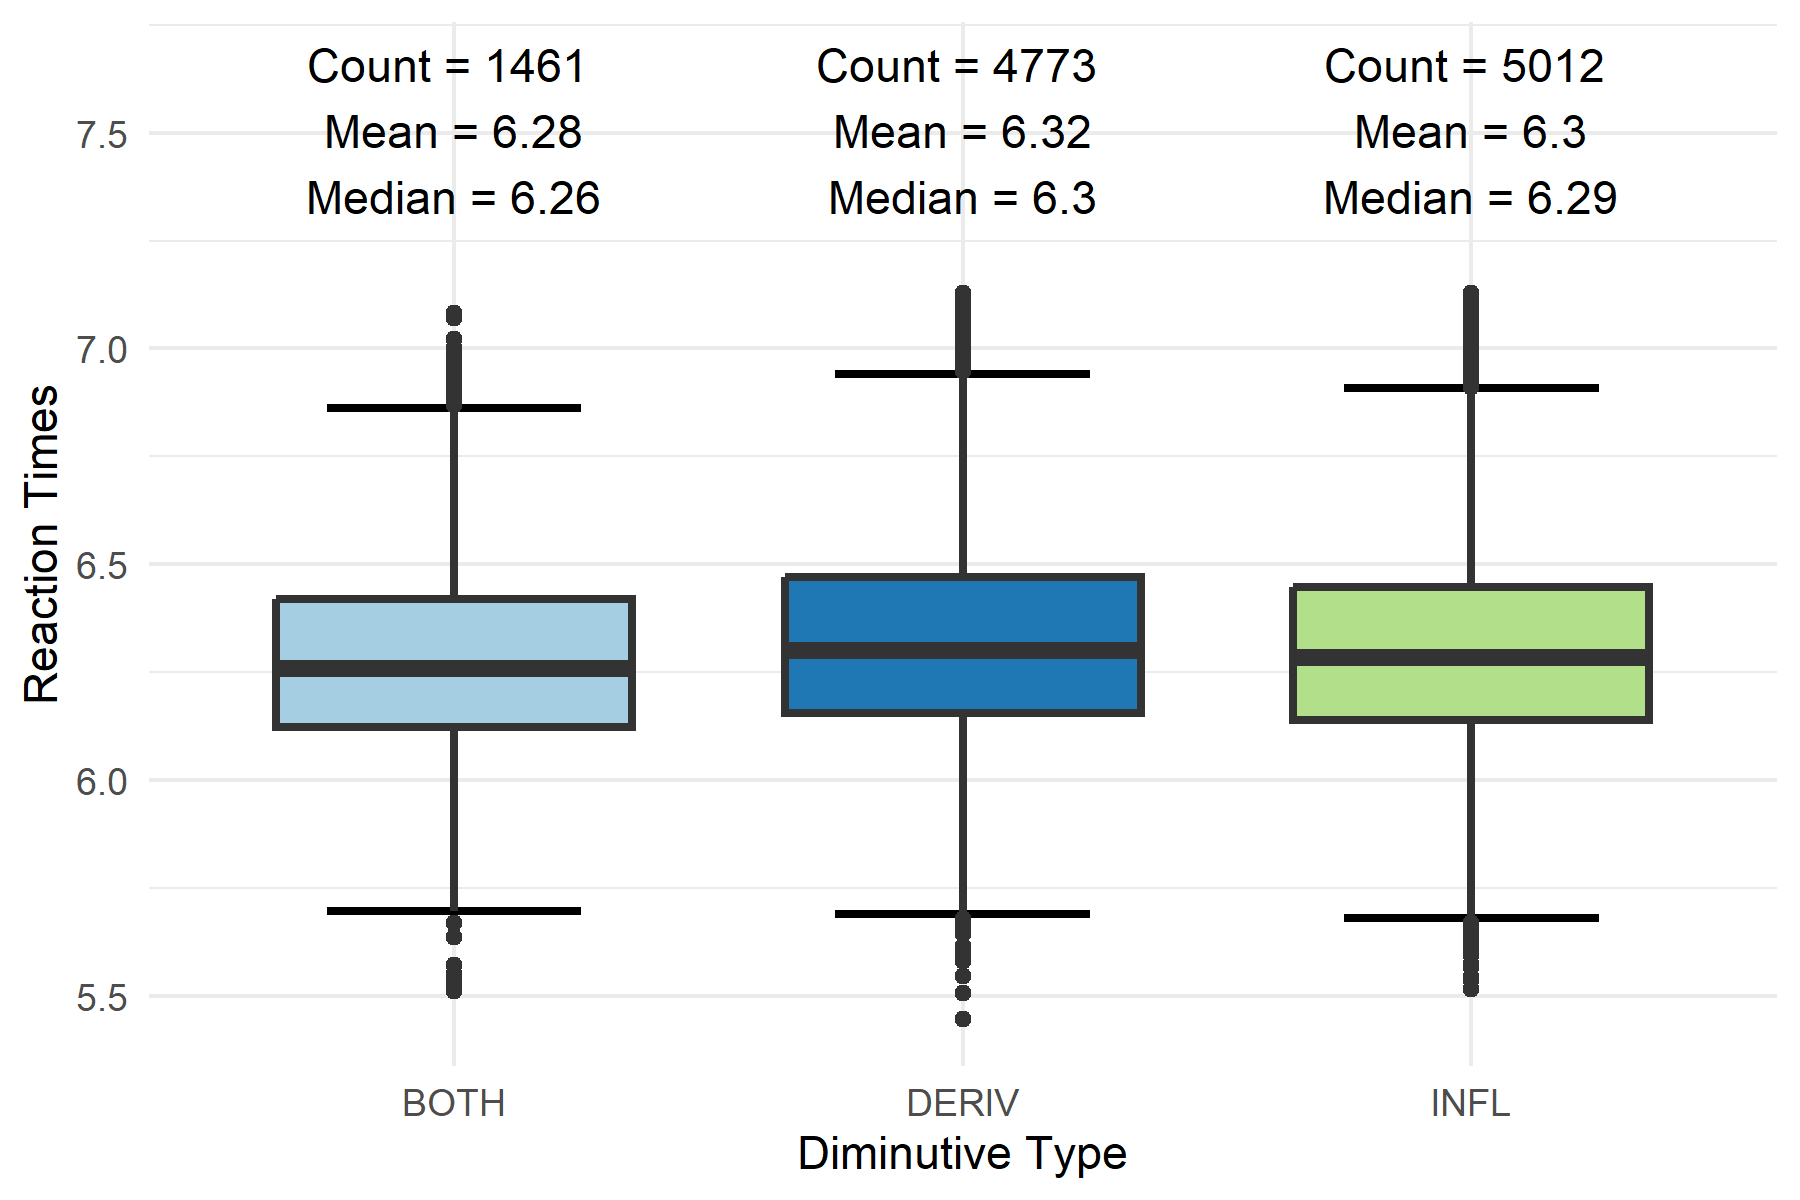
\includegraphics[width=\textwidth]{images/both_box.png}
    \caption[Exploratory boxplot for all diminutive types]{Exploratory boxplot for all diminutive types.}
    \label{fig:boxplot_both}
\end{figure}

An additional limitation stemming from both the choice of experiment and the theoretical background deserves a special mention. During the process of data selection, it was decided to exclude a group of items comprising diminutives with multiple structural interpretations. For example, the word \textit{gaat-je}, glossed as hole-DIM, accommodates both semantic patterns. In its semantically transparent, inflectional interpretation, it simply refers to a small hole of any kind, while the semantically opaque derivational interpretation comes with the specialised meaning of "tooth cavity". Given the intransparent nature of lexical decision experiments, it could not be clearly assumed that one interpretation would be the dominant one among participants: a person presented with such a diminutive would presumably have all possible interpretations made available to them. Assuming obligatory decomposition together with the functional split hypothesis, such a form would simultaneously produce two possible structures. However, it was not clear whether this would have a facilitatory effect on reaction times or an inhibitory one, as the two structures were assumed to enter in competition with one another. This would either result in longer reaction times due to an increase in cognitive load associated with processing two structures at once, or it would be enough for one of the structures, either the more frequently encountered or the less complex one, to reach the end of the recombination process and trigger a word recognition effect. 

Since a clear prediction could not be made with regards to effect on reaction times, all items assigned the value \texttt{both} for diminutive type were excluded from the analysis. However, after the results presented in Chapter~\ref{chp:study} were obtained and analysed, this additional group of items was reintroduced into the experimental dataset for an exploratory analysis. Surprisingly enough, the newly introduced group showed the lowest mean reaction times (mean raw RT = 551ms, compared to 562 for \texttt{infl} and 574 for \texttt{deriv}), with the log-transformed reaction times reflecting the same pattern and a series of pairwise t-tests establishing the difference in means as statistically significant (all $p$<0.05). Once again, the differences between groups are summarised in Figure~\ref{fig:boxplot_both}. An attempt was made to fit an experimental model using the same formula as the one in Chapter~\ref{chp:results} in order to investigate the effect of \textit{both} further; however, the model failed to converge. Nevertheless, the exploratory findings present an additional puzzle, one that the functional split proposal needs to take into account in order to achieve its goal of explaining the peculiar nature of diminutive morphology not just in Dutch, but in every language that patterns with it.

